\documentclass[10pt, twocolumn]{article}
\usepackage[utf8]{inputenc}
\usepackage[T1]{fontenc}
\usepackage{lmodern}
\usepackage{listings}
\usepackage{makeidx}
\usepackage[toc, page]{appendix}
\usepackage{float}
\usepackage{lscape}
\usepackage{csquotes}
\usepackage{soul}
\usepackage{textcomp}
\usepackage{gensymb}
\usepackage{pdfpages}
\usepackage{caption}
\usepackage{subcaption}
\usepackage{url}
\lstset{
	keywords={SELECT, WHERE, COLUMNS, ROWS, ON, MEMBER, WITH, FROM, ALL, CROSSJOIN, TOPCOUNT, ASC, DESC, AS, PARENT, CURRENTMEMBER, CHILDREN, PREVMEMBER, NEXTMEMBER, ORDER, RANK, GENERATE},
	keywordstyle=\color{red}\bfseries
}
% \usepackage{geometry}
\usepackage[left=25mm, right=25mm, top=30mm, bottom=30mm]{geometry}
\usepackage{rotating}
\usepackage[section]{placeins}
\usepackage{chngcntr,array}
\usepackage{graphicx}
\usepackage{lscape}
\usepackage{dirtree}
\usepackage[
	breaklinks=true,
	colorlinks=true,
	linkcolor=blue,
	urlcolor=blue,
	citecolor=blue,
	bookmarks=true,
	bookmarksopenlevel=2
]{hyperref}
\usepackage{xcolor}
\usepackage{algorithm}
\usepackage{algpseudocode}
\usepackage{amsmath}
\usepackage{amsfonts}
\usepackage{amssymb}
\usepackage{indentfirst}

\title{
	Machine Learning
	\\-\\
	Markov Decision Processes and Reinforcement Learning
}
\author{
	\href{mailto:brandon.alves@gatech.edu}{Brandon Alves}
}
\date{\today}

\begin{document}
	\maketitle
	\thispagestyle{empty}
	\tableofcontents
	% \listoffigures
	% \clearpage
	% \setcounter{page}{1}
	\section{Introduction}
		In this report I will explore the Markov Decision Processes (MDP). Instead of learning from data either supervised or unsupervised, here, we will discuss the notion of making decisions and how an agent can evolve in its environment. For that we first need to modelise the environment and the agent. A MDP is defined as the following:
		\begin{itemize}
			\item A set of states $S$.
			\item A set of actions $A(s)$ that can be taken in each state $s \in S$.
			\item A transition model $T(s, a, s') = P(s' | s, a)$ that describes the probability of transitioning from state $s$ to state $s'$ when taking action $a$.
			\item A reward function $R(s)$ that gives the reward for being in state $s$.
			\item A discount factor $\gamma$ that determines the importance of future rewards.
		\end{itemize}
		Given that MDP defined above and an initial state $s_0$, the goal is to find a policy $\pi$ that maximizes the expected return in order to choose the best action at each state. The expected return is defined as:
		\begin{equation}
			G_t = \sum_{k=0}^{\infty} \gamma^k R_{t+k+1}
		\end{equation}
		Where $G_t$ is the expected return starting at time $t$ and $R_{t+k+1}$ is the reward at time $t+k+1$. The discount factor $\gamma$ is used to determine the importance of future rewards. If $\gamma = 0$, then the agent will only consider the immediate reward. If $\gamma = 1$, then the agent will consider all future rewards the same way.
		The policy $\pi(s) \rightarrow a$ tells the agent what action to take in each state. The policy can be deterministic or stochastic. The optimal policy $\pi^{\star}$ is a policy that maximizes the expected return. An optimal policy is not always known, so we need to find it. An optimal policy can be found using the Bellman equation:
		\begin{equation}
			U(s) = R(s) + \gamma max_{a \in A(s) }\sum_{s' \in S} T(s, a, s') U(s')
		\end{equation}
		Where $U(s)$ is the utility of being in state $s$. The utility of a state is the expected return starting from that state. The Bellman equation can be used to find an optimal policy $\pi^{\star}$ by iterating over all states and actions. There is two main algorithms to find an optimal policy : Value Iteration and Policy Iteration. The Value Iteration algorithm find an optimal policy by calculating the utility of each state using the Bellman equation. Bellman equation gives us one equation per state, however the maximum operator does not permit to solve a linear system of $n$ equations for $n$ unknowns. Therefore Value Iteration uses an iterative method to find the optimal policy:
		\begin{enumerate}
			\item Initialize random utilities for each state;
			\item Update the utilities based on neighboring states;
			\item Repeat the update until convergence;
			\item Get an optimal policy: $\pi^{\star}(s) = argmax_{a \in A(s)} \sum_{s' \in S} T(s, a, s') U(s')$.
		\end{enumerate}
		The Policy Iteration algorithm is similar to the Value Iteration algorithm, but instead of updating the utilities of each state, it updates the policy. The algorithm is as follows:
		\begin{enumerate}
			\item Initialize random policy;
			\item Evaluate the utility of each state given the policy: $U(s) = R(s) + \gamma \sum_{s' \in S} T(s, \pi(s), s') U(s')$;
			\item Improve the policy: $\pi^{\star}(s) = argmax_{a \in A(s)} \sum_{s' \in S} T(s, a, s') U(s')$;
			\item Repeat the evaluation and improvement process until convergence.
		\end{enumerate}

		We chose Q-Learning as our reinforcement learning algorithm. Q-Learning is a model-free reinforcement learning algorithm. That means that the agent does not learn the transistion model nor the reward function. Instead, the agent discovers which actions are good or bad by interacting with the world. MDPs are easy to solve because we know everything about them (states, actions, rewards, and transition model). In that case, we will not know anything about the transition model and reward function. We still want learn the optimal policy. The fundamental tradeoff of Reinforcement Learning is exploration vs exploitation. Rather than learning the utility of a state, we will learn a new function, $Q(s, a)$. Each time we interact with the world we gain an experience. From that experience, we can learn a policy. We define:
		\begin{itemize}
			\item $<s, a, s', r>$ : experience tuple.
			\item $Q(s, a) = R(s) + \gamma max_{a' \in A(s)} Q(s', a')$.
			\item $Q(s, a)$ : expected immediate reward for taking action $a$ in state $s$ plus the sum of discounted rewards for acting optimally afterward (in the future, according to Q)
			\item $Q(s, a) = (1 - \alpha) Q(s, a) + \alpha (r + \gamma max_{a' \in A(s)} Q(s', a'))$ : Q-Learning update rule.
		\end{itemize}
		Q-Learning algorithm is as follows:
		\begin{enumerate}
			\item Initialize $Q$ (zeros, or small random numbers near zero)
			\item Act and observe an experience tuple $<s, a, s', r>$
			\item Update Q according to the update rule
			\item Repeat
		\end{enumerate}

		In this report, we will first solve the MDP problems using Value Iteration (VA) and Policy Iteration (PI) to find an optimal policy, given the transition model and the reward model. Then, we will use Q-Learning, a model free reinforcement learning algorithm, to learn an optimal policy.
	\section{Problems}
		In this article, I will discuss the following MDP problems:
		\begin{itemize}
			\item Grid World
			\item Block Dude
		\end{itemize}
		\subsection{Grid World}
			Grid World is a simple MDP problem where the agent is in a grid and can move in four directions: forward, backward, left and right. The agent cannot move diagonally. The grid is a $n$ by $n$ matrix where $n$ is the size of the grid. The states are represented by the coordinates of the agent in the grid. The actions are represented by the direction the agent can move. Actions can either be deterministic or stochastic. The agent starts at the left bottom corner of the grid and the goal is to reach the right top corner of the grid. A certain number of obstacles can also be present in the grid. The agent cannot move through an obstacle. Taking an action that would move the agent through an obstacle or outside the grid will result in the agent staying in the same state.

			I found Grid World as an interesting problem because it is simple and easy to understand. It has a relative small state space and action space that permits to converge to the optimal policy with less than 50 iterations. It can therefore be used as a benchmark to test other MDP problems. Also Grid World has many parameters that can be tuned. The parameters that can be tuned are:
			\begin{itemize}
				\item The size of the grid.
				\item The number of obstacles.
				\item The probability of going into a specific direction when taking an action.
			\end{itemize}
			Therefore it will be interesting to see how the results change when changing the parameters.
		\subsection{Block Dude}
			Block Dude is a MDP implementation of the \href{https://fr.wikipedia.org/wiki/Block_Dude}{Block Dude} puzzle game. The agent is a dude that can move in three directions: left, right and up in the case that the platform in front of the dude is one level above. The player can also move blocks that are present in the different platforms. He can only carry one block at the time to move it. The actions are represented by the direction the agent can move as well as pick up and put down actions for moving blocks. The purpose of Block Dude is to reach a door.

			I found Block Dude as an interesting problem because it is more complex than Grid World. It has a larger state space and action space. The number of iteration needed to converge increases as the level increases. In addition, that kind of problem is very similar to real life problems. For example, in a warehouse, the agent can be a robot that can move in different directions and pick up and put down objects. Therefore, it would be interesting to see how the agent can learn to solve this kind of problem.
	\section{Markov Decision Processes}
		\subsection{Value and Policy Iteration - Grid World}
			\subsubsection*{Introduction}
				In this section we will solve Grid World (GW) MDP either using Value Iteration (VA) or Policy Iteration (PI). We will also compare the results of the two methods. For GW, we will discuss the influence of the following parameters:
				\begin{itemize}
					\item The size of the grid;
					\item The stochastic success probability of the actions;
					\item The percentage of obstacles in the grid;
					\item The reward value for reaching the goal;
					\item The discount factor.
				\end{itemize}
				We present on figure \ref{fig:GW:iterations} the results of the number of iterations needed to converge to an optimal policy according to the parameters of the Grid World problem.

				\begin{figure}[]
					\centering
					\begin{subfigure}[t]{0.49\textwidth}
						\centering
						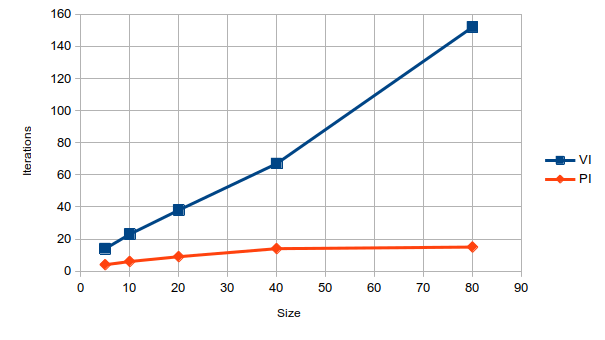
\includegraphics[width=.7\textwidth]{../graphics/GridWorld_size_iterations.png}
						\caption{Number of iterations according to the size of the grid.}
						\label{fig:GW:size}
					\end{subfigure}
					\begin{subfigure}[t]{0.49\textwidth}
						\centering
						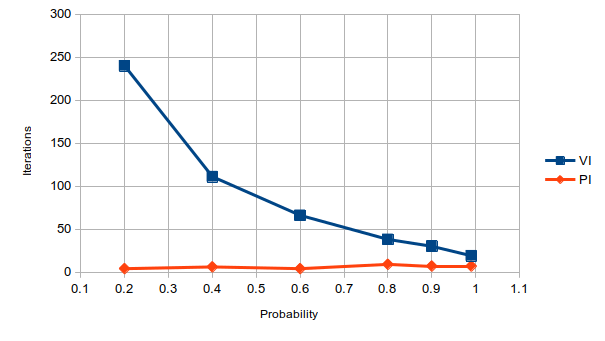
\includegraphics[width=.7\textwidth]{../graphics/GridWorld_probability_iterations.png}
						\caption{Number of iterations according to the stochastic success probability of the actions.}
						\label{fig:GW:probability}
					\end{subfigure}
					\begin{subfigure}[t]{0.49\textwidth}
						\centering
						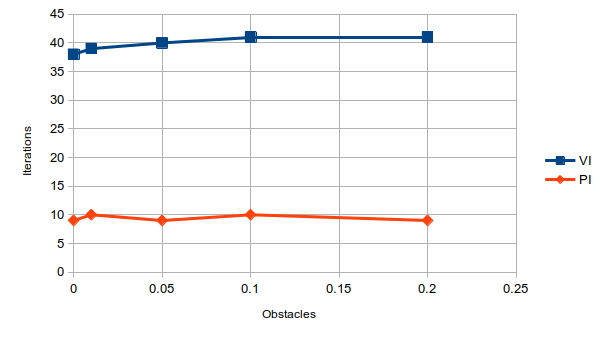
\includegraphics[width=.7\textwidth]{../graphics/GridWorld_obstacles_iterations.png}
						\caption{Number of iterations according to the percentage of obstacles in the grid.}
						\label{fig:GW:obstacles}
					\end{subfigure}
					\begin{subfigure}[t]{0.49\textwidth}
						\centering
						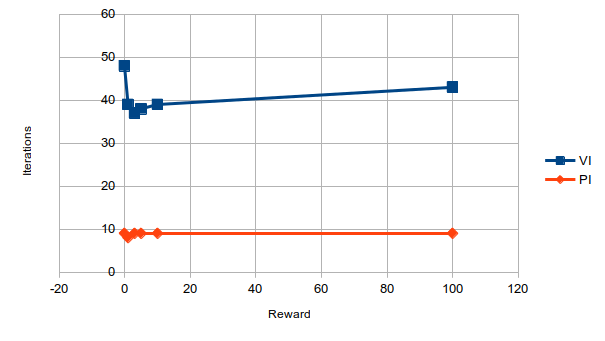
\includegraphics[width=.7\textwidth]{../graphics/GridWorld_reward_iterations.png}
						\caption{Number of iterations according to the reward value for reaching the goal.}
						\label{fig:GW:reward}
					\end{subfigure}
					\begin{subfigure}[t]{0.49\textwidth}
						\centering
						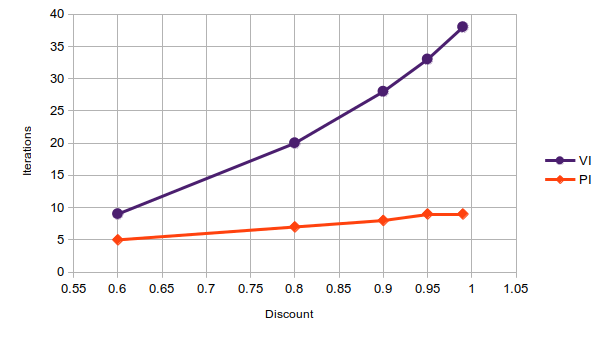
\includegraphics[width=.7\textwidth]{../graphics/GridWorld_discount_iterations.png}
						\caption{Number of iterations according to the discount factor.}
						\label{fig:GW:discount}
					\end{subfigure}
					\caption{Number of iterations to converge to an optimal policy according to the parameters of the Grid World problem.}
					\label{fig:GW:iterations}
				\end{figure}
			\subsubsection*{Grid Size}
				We can see on figure \ref{fig:GW:size} the evoluation of the number of iteration needed to find an optimal policy according to the size of the grid. As we can see, the number of iterations increases with the size of the grid. This is because the state space is definined by the size of the grid: the number of states is equal to the number of cells in the grid. It is interesting to notice that while, with VI, the number of iterations seems to increase exponentially with the size of the grid, with PI, the number of iterations seems to increase logarithmically with the size of the grid. However we have to notice that PI takes much longer than VI in terms of time to converge. The fact that VI converges faster than PI can be explained by the fact that within each iterations, VI updates  the utility of each state based on the neighbor states while PI considers all the states at once. Therefore, PI is more efficient in terms of iteration than VI but takes more time to converge.

				We present on figure \ref{fig:GW:size:comparison} an optimal policy for both VI and PI for a 20x20 grid. We can see that most of the actions and utilities are consistent but some minor differences results from the fact that there are many optimal solutions for this problem.

				\begin{figure}[]
					\centering
					\begin{subfigure}[t]{0.24\textwidth}
						\centering
						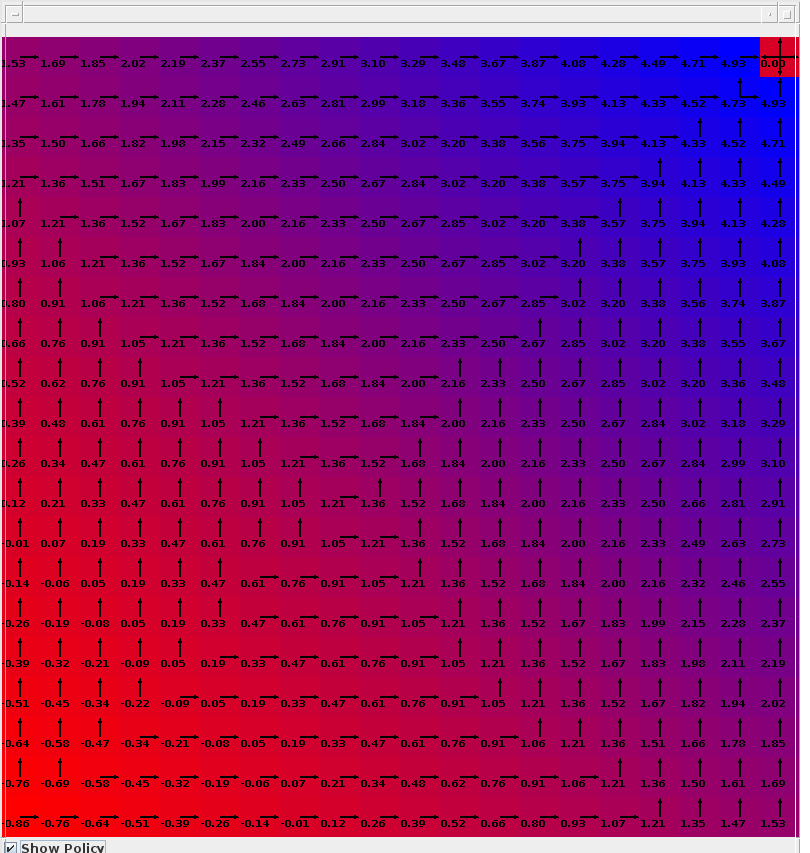
\includegraphics[width=\textwidth]{../graphics/GridWorld_20_vi_size.png}
						\caption{Value Iteration}
						\label{fig:GW:size:VI}
					\end{subfigure}
					\begin{subfigure}[t]{0.24\textwidth}
						\centering
						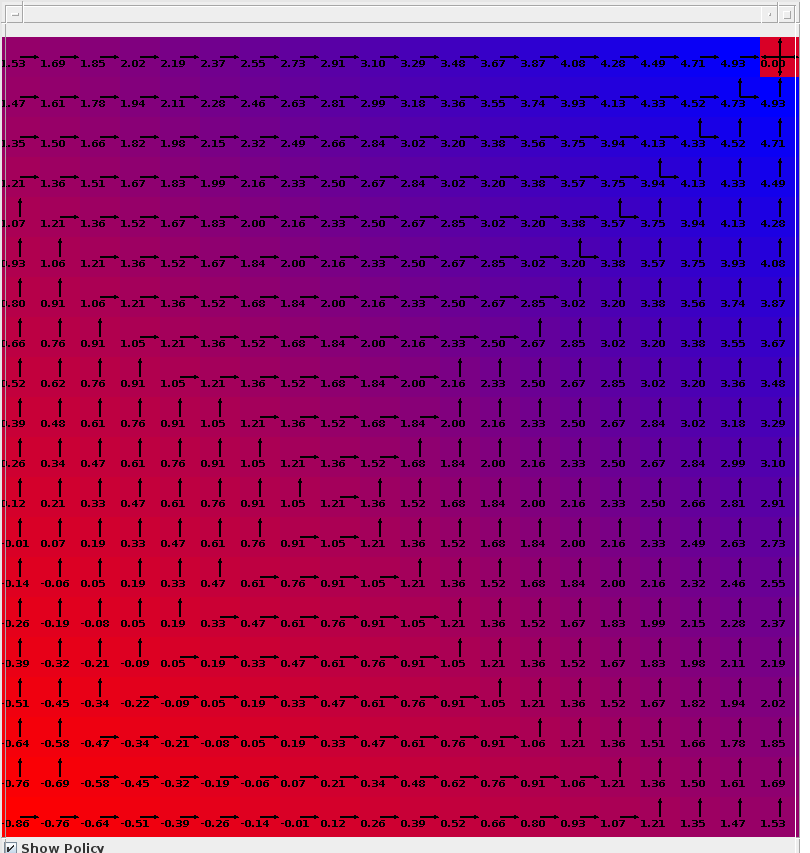
\includegraphics[width=\textwidth]{../graphics/GridWorld_20_pi_size.png}
						\caption{Policy Iteration}
						\label{fig:GW:size:PI}
					\end{subfigure}
					\caption{Optimal policy for a 20x20 Grid World problem.}
					\label{fig:GW:size:comparison}
				\end{figure}
			\subsubsection*{Stochastic Success Probability}
				We can see on figure \ref{fig:GW:probability} the evoluation of the number of iteration needed to find an optimal policy according to the stochastic success probability of the actions. As we can see, the number of iterations decreases when the probability increases with VI but is not affected with PI. This is explained by the fact that in PI, we still have to evaluate the utility of each state, while in VI, we only have to evaluate the utility of the neighbor states. The large number of possible shortest paths slows down the converging process of PI. Therefore, less there is uncertainty, more the convergence is faster.

				We can see on figure \ref{fig:GW:probability:comparison} an optimal policy for both VI and PI for a 20x20 grid with a stochastic success probability of 0.6. As we can see, optimal policies are very similar, they only differ on the diagonal. PI handles better the uncertainty of the actions than VI, in terms of efficiency. This is because PI evaluates the actions directly while VI does not. VI only evaluates the utility of the neighbor states. When the probability decreses, VI will have higher chance to go in a wrong direction.

				Another interesting fact, but not displayed here, is that when the probability decreases to 0.2, an optimal policy will suggest to go to the opposite direction of the goal. That is beacuse going in that opposite direction will have a higher probability of going to the goal. This is a very interesting fact that shows the importance of the stochastic success probability of an optimal policy.

				\begin{figure}[]
					\centering
					\begin{subfigure}[t]{0.24\textwidth}
						\centering
						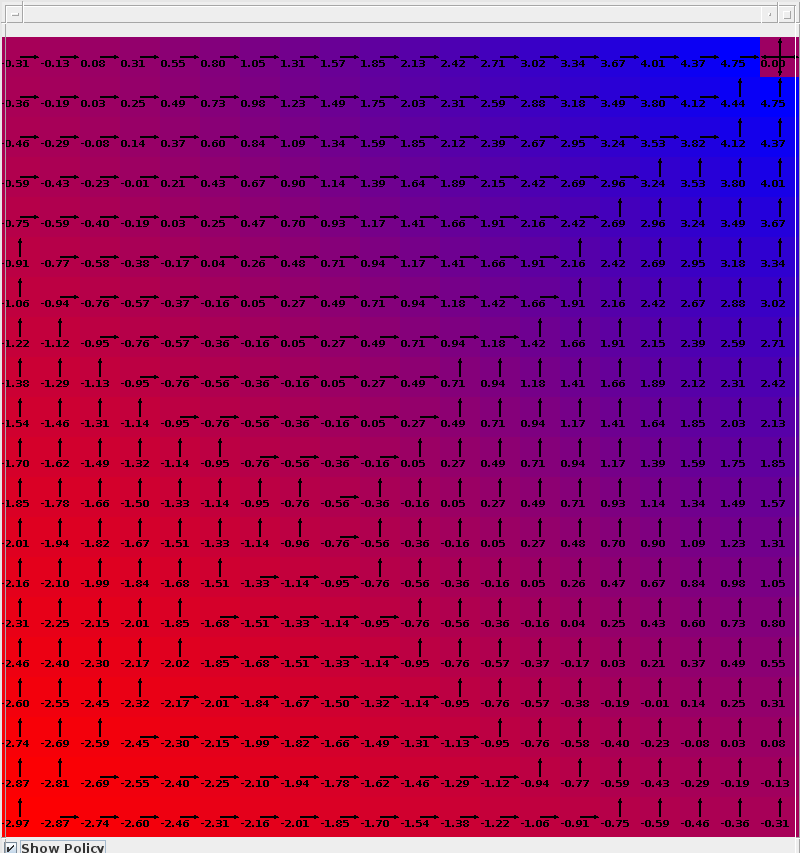
\includegraphics[width=\textwidth]{../graphics/GridWorld_0.6_vi_prob.png}
						\caption{Value Iteration}
						\label{fig:GW:probability:VI}
					\end{subfigure}
					\begin{subfigure}[t]{0.24\textwidth}
						\centering
						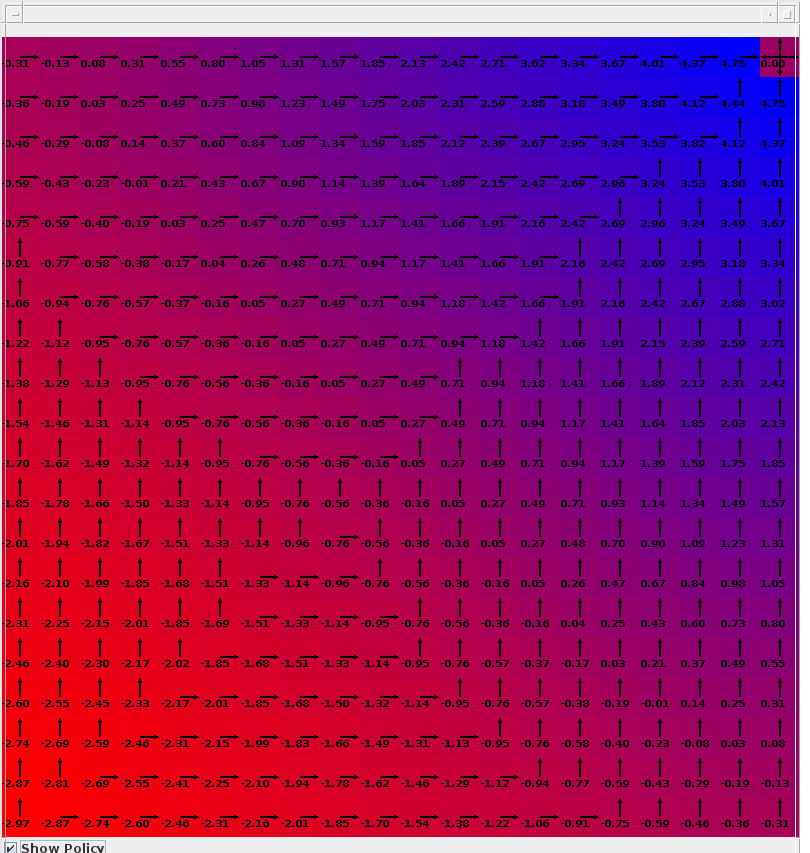
\includegraphics[width=\textwidth]{../graphics/GridWorld_0.6_pi_prob.png}
						\caption{Policy Iteration}
						\label{fig:GW:probability:PI}
					\end{subfigure}
					\caption{Optimal policy for a 0.6 success probability Grid World problem.}
					\label{fig:GW:probability:comparison}
				\end{figure}
			\subsubsection*{Percentage of Obstacles}
				We present on figure \ref{fig:GW:obstacles} the evoluation of the number of iteration needed to find an optimal policy according to the percentage of obstacles in the grid.
				It is interesting to constate that the number of iterations is not really affected by the percentage of obstacles with VI and PI. That can be explained by the fact that obstacles are not considered as states. Therefore, the number of states is not \textit{significantly} affected by the percentage of obstacles. However, the runing time is well affected by the percentage of obstacles. The more obstacles we have, the less states we have and therefore the faster the algorithm will converge.

				We can see on figure \ref{fig:GW:obstacles:comparison} an optimal policy for both VI and PI for a 20x20 grid with a 20\% of obstacles. That time, we can see that the optimal policies are exactly the same. This can be explained by the fact that obstacles introduced some constraints on the action space. Those constraints led to less stochasticity in the actions.
				\begin{figure}[]
					\centering
					\begin{subfigure}[t]{0.24\textwidth}
						\centering
						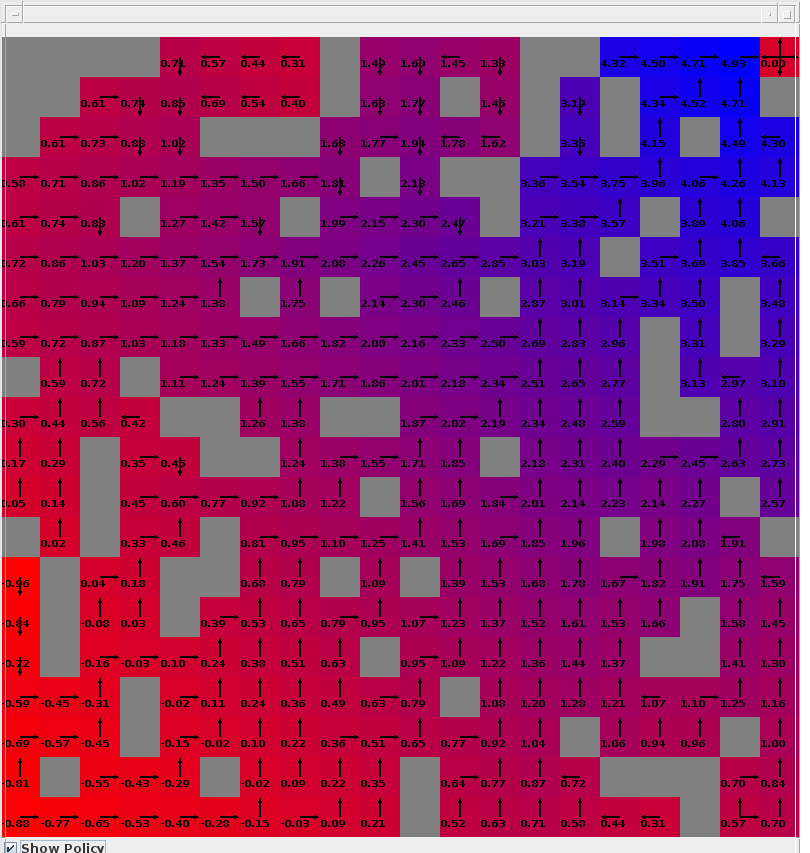
\includegraphics[width=\textwidth]{../graphics/GridWorld_0.2_vi_wallpercent.png}
						\caption{Value Iteration}
						\label{fig:GW:obstacles:VI}
					\end{subfigure}
					\begin{subfigure}[t]{0.24\textwidth}
						\centering
						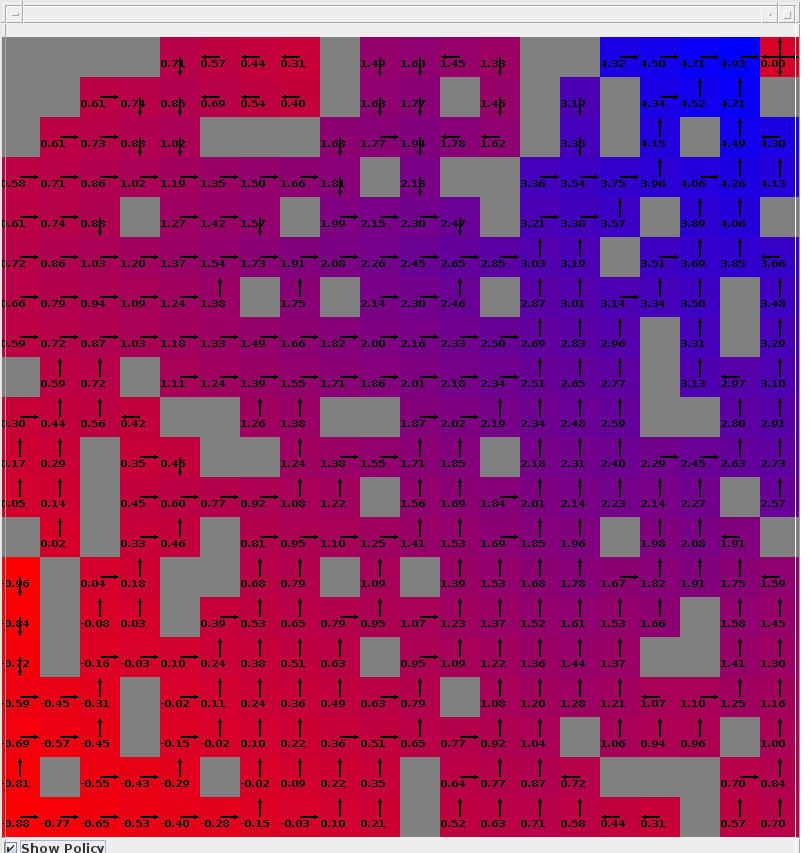
\includegraphics[width=\textwidth]{../graphics/GridWorld_0.2_pi_wallpercent.png}
						\caption{Policy Iteration}
						\label{fig:GW:obstacles:PI}
					\end{subfigure}
					\caption{Optimal policy for a 0.2 wall appearance percent Grid World problem.}
					\label{fig:GW:obstacles:comparison}
				\end{figure}
			\subsubsection*{Reward Value}
				We present on figure \ref{fig:GW:reward} the evoluation of the number of iteration needed to find an optimal policy according to the reward value for entering into the final location. The default reward value for all the other states is -0.1. That is why we started with reward for reaching the goal of -0.1. As we can see, with VI, the number of iteration with a reward of -0.1 is very high. That was to be expected. Indeed, in that case, only the states near the final one know to reach the goal but all other states do not have a tendency because they only updates the value function based on their neighbors. That leads to a very slow convergence. However, when the reward is different from the other states, the convergence is faster.

				The evolution of the number of iterations for VI is interesting. It first decreases from a high value because of what we already explained to reach a minimum for a reward of 3, to increase afterwards. I do not know why. Indeed, a high reward for reaching the goal should lead to a faster convergence.

				It is interesting to see that for PI, the number of iterations is not affected by the reward value. That is because, in PI, we do not update the utility of each state like in VI, but we update the policy. Therefore, the reward value does not really afects the number of iterations.

				As we can see on figure \ref{fig:GW:reward:comparison}, results for VI and PI mostly agree with each other with a reward value of 3.

				\begin{figure}[]
					\centering
					\begin{subfigure}[t]{0.24\textwidth}
						\centering
						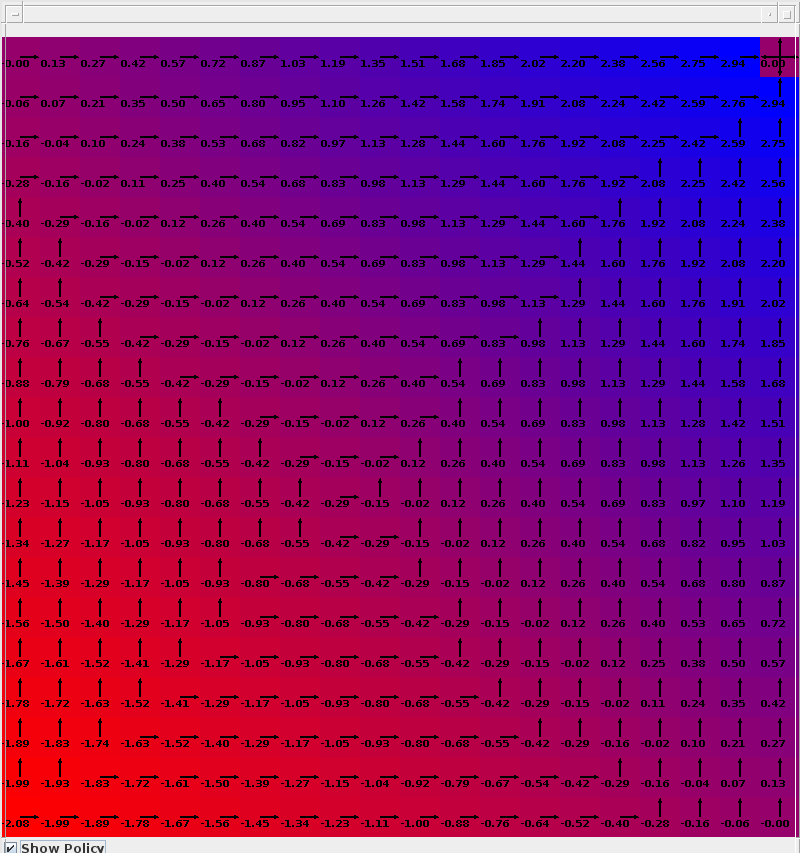
\includegraphics[width=\textwidth]{../graphics/GridWorld_3.0_vi_reward.png}
						\caption{Value Iteration}
						\label{fig:GW:reward:VI}
					\end{subfigure}
					\begin{subfigure}[t]{0.24\textwidth}
						\centering
						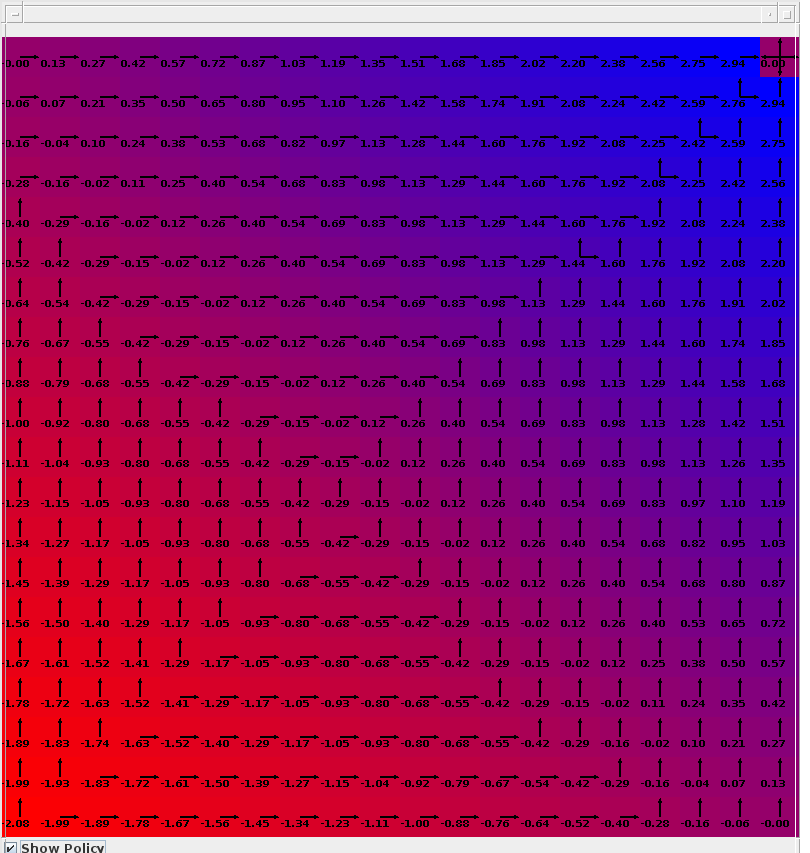
\includegraphics[width=\textwidth]{../graphics/GridWorld_3.0_pi_reward.png}
						\caption{Policy Iteration}
						\label{fig:GW:reward:PI}
					\end{subfigure}
					\caption{Optimal policy for a 3.0 reward value Grid World problem.}
					\label{fig:GW:reward:comparison}
				\end{figure}
			\subsubsection*{Discount Factor}
				We present on figure \ref{fig:GW:discount} the evoluation of the number of iteration needed to find an optimal policy according to the discount factor. As we already said, the discount factor reflects the importance of future rewards. The higher the discount factor, the more the agent will care about future rewards. We can see that the number of iterations is highly affected by the discount factor. The higher the discount factor, the lower the algorithm will converge. Which is logical because the agent will care more about future rewards and therefore will take more iterations to converge. However when having a small discount factor value, which means we are willing to take short term gains instead long term gains, we end up not finding an optimal policy because the states near starting position will not be incited to move toward the final location. Only the states near the final location enters in it because of the short term feedback. That is similar whith the case when we have very small value for the reward for VI. Large discount factor values take more time and iterations to converge for both VI and PI. It is fair in the sense that we are taking long term information into account. In the worst case the number of iterations grows polynomially in $\frac{1}{1- \gamma}$, so the convergence rate slows considerably as the discount value approaches 1.

				We can see on figure \ref{fig:GW:discount:comparison} that VI and PI found the same optimal policy again for a 0.9 discount factor.

				\begin{figure}[]
					\centering
					\begin{subfigure}[t]{0.24\textwidth}
						\centering
						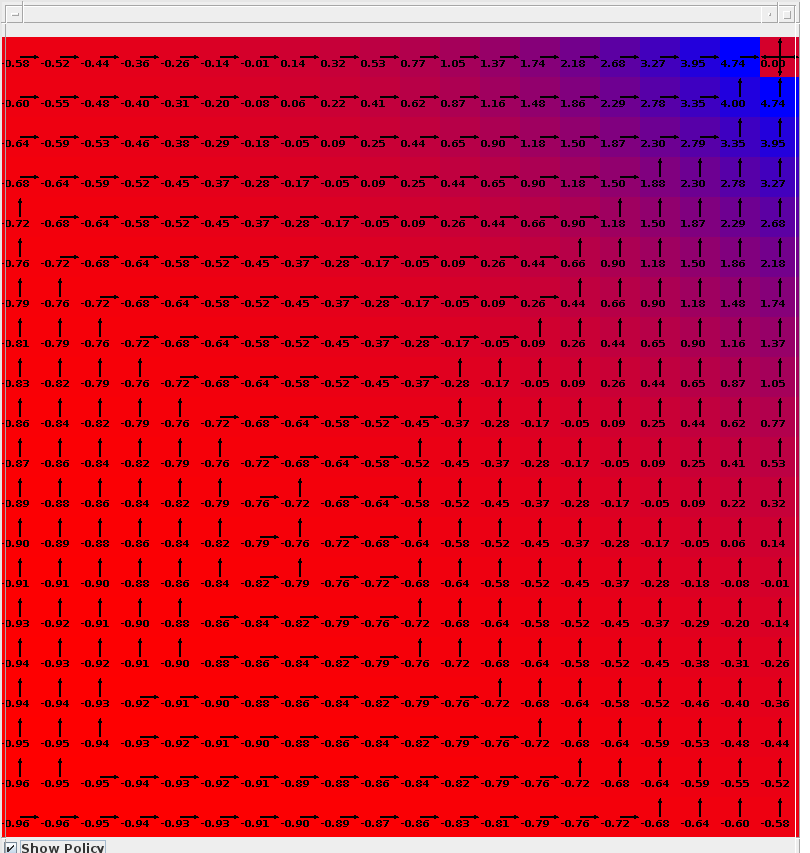
\includegraphics[width=\textwidth]{../graphics/GridWorld_0.9_vi_discount.png}
						\caption{Value Iteration}
						\label{fig:GW:discount:VI}
					\end{subfigure}
					\begin{subfigure}[t]{0.24\textwidth}
						\centering
						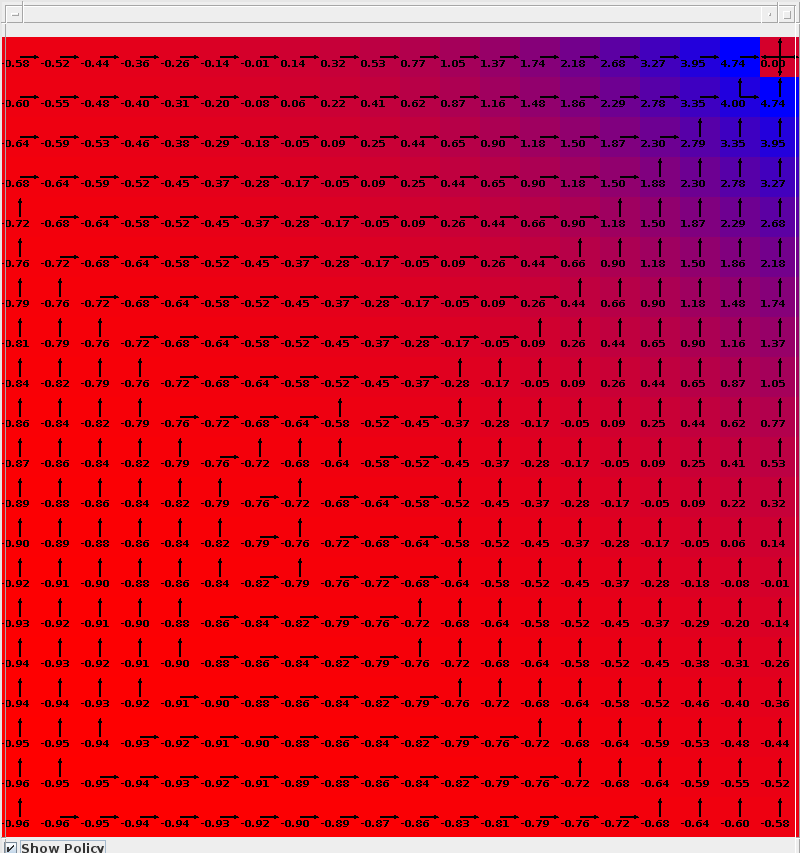
\includegraphics[width=\textwidth]{../graphics/GridWorld_0.9_pi_discount.png}
						\caption{Policy Iteration}
						\label{fig:GW:discount:PI}
					\end{subfigure}
					\caption{Optimal policy for a 0.9 discount factor Grid World problem.}
					\label{fig:GW:discount:comparison}
				\end{figure}
			\subsubsection*{Conclusion}
				We saw with the Grid World problem that the number of iterations needed to find an optimal policy is highly affected by the number of states for both VI and PI, the stochastic success probability of the actions for VI, the reward for VI and the discount factor for both VI and PI. We also saw that both VI and PI always success to find an optimal which is not always the same for both algorithms.
		\subsection{Value and Policy Iteration - Block Dude}
			\subsubsection*{Introduction}
				In this section we will solve Block Dude (BD) MDP either using Value Iteration (VA) or Policy Iteration (PI). We will also compare the results of the two methods. For BD, we will discuss the influence of the following parameters:
				\begin{itemize}
					\item The level of the game;
					\item The reward value for reaching the goal;
					\item The discount factor.
				\end{itemize}
				We present on figure \ref{fig:BD:iterations} the results of the number of iterations needed to converge to an optimal policy according to the parameters of the Block Dude problem.

				\begin{figure}[]
					\centering
					\begin{subfigure}[t]{0.49\textwidth}
						\centering
						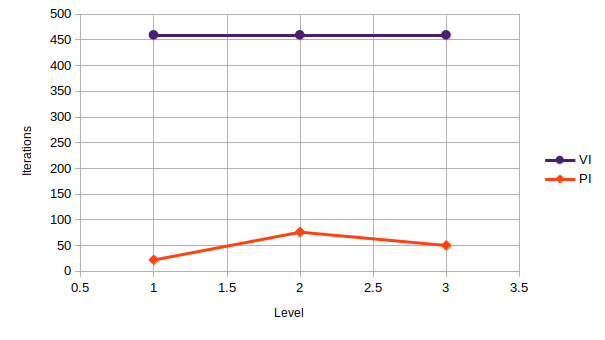
\includegraphics[width=.7\textwidth]{../graphics/BlockDude_level_iterations.png}
						\caption{Number of iterations according to the level of the game.}
						\label{fig:BD:level}
					\end{subfigure}
					\begin{subfigure}[t]{0.49\textwidth}
						\centering
						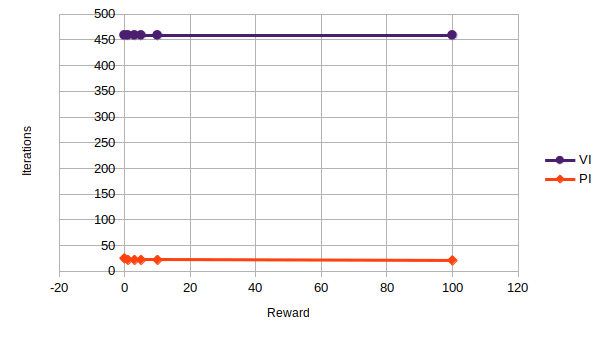
\includegraphics[width=.7\textwidth]{../graphics/BlockDude_reward_iterations.png}
						\caption{Number of iterations according to the reward value for reaching the goal.}
						\label{fig:BD:reward}
					\end{subfigure}
					\begin{subfigure}[t]{0.49\textwidth}
						\centering
						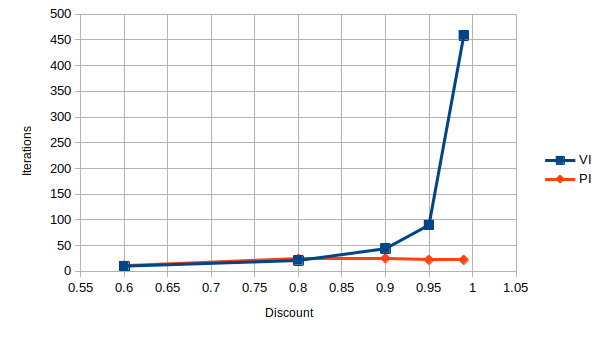
\includegraphics[width=.7\textwidth]{../graphics/BlockDude_discount_iterations.png}
						\caption{Number of iterations according to the discount factor.}
						\label{fig:BD:discount}
					\end{subfigure}
					\caption{Number of iterations to converge to an optimal policy according to the parameters of the Grid World problem.}
					\label{fig:BD:iterations}
				\end{figure}
			\subsubsection*{Level}
				We can see on figure \ref{fig:BD:level} the evolution of the number of iterations needed to find an optimal policy according to the level of the game. The level of BD problem reflects the maximal length columns of blocks we have to create to reach the goal. In general, the higher the level, the more difficult the problem is. However, higer level does not mean higher number of states. For example, the level 1 has 840 states, level 2 has 230995 states and level 3 has 14199 states. In that case, we generated a 2-level BD problem that has the most number of states compared with the 1-level and 3-level game we generated. It is interesting to see that, unlike for GW problem, the number of states did not affect the number of iterations needed to find an optimal policy for VI. However, the runing time of VI does increase with the number of iterations. The fact that the runing time increases with the number of states is explained by the fact in VI, within each iterations we have to compute the value of each state. It would have been interesting to see if, by testing with another values of number of states for BD problem, we would have obtained the same observations as for GW problem. However, the runing time was too high with BD problem to allow us to test with a large number of states. For PI, we got the same results as for VI. The number of iterations needed to find an optimal policy as well as the running time increases with the number of states.
			\subsubsection*{Reward Value}
				We can see on figure \ref{fig:BD:reward} the evolution of the number of iterations needed to find an optimal policy according to the reward value for reaching the goal. We can see that the number of iterations needed to find an optimal policy is not affected by the reward value. That time the number of iterations is constant for all reward values. We are having very different results with VI compared to GW problem. It seems that VI is more sensitive to the problem modelisation than PI. Unlike in GW, a large reward value does practically have more impact on the states that are far from the final state than a smaller reward value. For PI, we got the same results as for GW : both number of iteration and running time independant of the reward value.
			\subsubsection*{Discount Factor}
				We present on figure \ref{fig:BD:discount} the evolution of the number of iterations needed to find an optimal policy according to the discount factor. We can see that those results are consistant with what we obtained for GW : smaller discount factor value only takes short term gain into account and as a result the resulting policy does not lead the agent to the goal wheras with higher discount factor value, the run time and iterations to converge increase significantly, but the policy converges to an optimal solution.
			\subsubsection*{Conclusion}
				For BD problem it was difficult to compare the actions of the optimal policy due to the high number of states.

				To summarise, we saw that small number of states and small discount factor value will yield higher convergence rate. However, small discount factor value may not yield to an optimal policy. Reward and probability of transition are not the most decisive factors for the convergence. VI convergences slower that PI in terms of interations, while VI converges faster than PI in terms of run time.
	\section{Reinforcement Learning}
		\subsection*{Introduction}
			We use Q-learning (QL) as our Reinforcement Learning (RL) algorithm to solve both GW and BD. We evaluate the performance of QL based on two metrics :
			\begin{itemize}
				\item the number of steps per episode,
				\item the average reward per episode.
			\end{itemize}
			The number of steps per episode metric gives us when QL converges and in how many steps it does. The average reward per episode metric gives us the increase of reward related to each episode and converges to the reward value of the optimal solution. In this way, we have a direct view of QL learning from the past episodes. Moreover, we can compare the final reward value with the results we got from the past section.

			In that section, we will also see the impact of the following parameters to help us understanding better QL:
			\begin{itemize}
				\item The initial Q value;
				\item The epsilon value;
				\item The learning rate.
			\end{itemize}
		\subsection{Q-Learning - Grid World}
			The results in terms of time with the different initial Q values, epsilon values and learning rate values are present in figure \ref{fig:GW:QL}. The best performance of initial Q value is obtained with 0.3 and worst with 30. The best performance of epsilon value is obtained with 0.05 and worst with 0.8. The best performance of learning rate value is obtained with 0.5 and worst with 0.01.

			\begin{figure}[]
				\centering
				\begin{subfigure}[t]{0.49\textwidth}
					\centering
					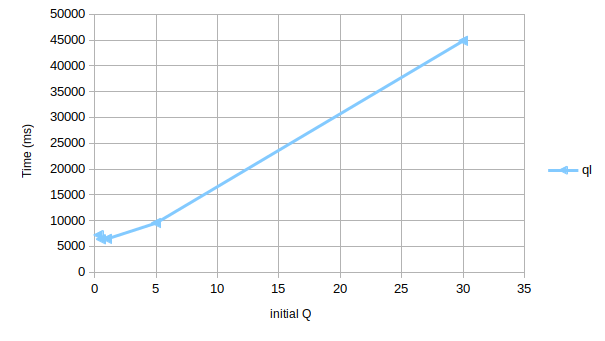
\includegraphics[width=\textwidth]{../graphics/GridWorld_qinit_time.png}
					\caption{Time according to the initial Q value.}
					\label{fig:GW:qinit}
				\end{subfigure}
				\begin{subfigure}[t]{0.49\textwidth}
					\centering
					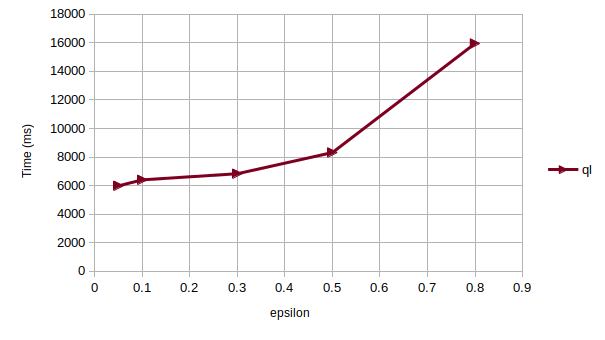
\includegraphics[width=\textwidth]{../graphics/GridWorld_epsilon_time.png}
					\caption{Time according to the epsilon value.}
					\label{fig:GW:epsilon}
				\end{subfigure}
				\begin{subfigure}[t]{0.49\textwidth}
					\centering
					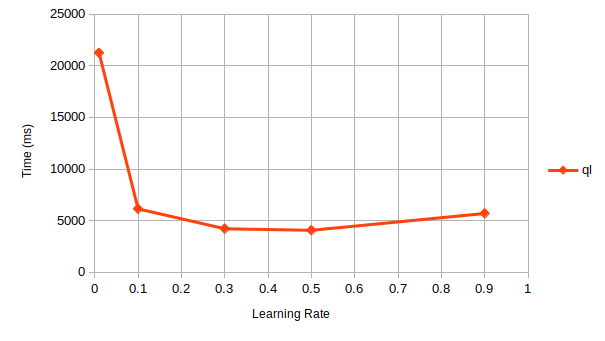
\includegraphics[width=\textwidth]{../graphics/GridWorld_rate_time.png}
					\caption{Time according to the the learning rate.}
					\label{fig:GW:rate}
				\end{subfigure}
				\caption{Number of iterations to converge to an optimal policy according to the parameters of the Grid World problem.}
				\label{fig:GW:QL}
			\end{figure}

			QL needs random restart to avoid the problems caused by the greedy action selection strategy.  If we do not use random restart, we will mostly use what we already know. We will always choose the same action and therefore quickly converge to a local minima. So we implement epsilon greedy exploration which is very similar to simulated annealing. Epsilon is the decaying factor for cooling down the temperature and initial Q values are just the initial temperature in terms of simulated annealing. With lower epsilon value, QL will choose the action even it is not the best action to take. Lower epsilon value means cooling the temperature slower and do more exploration. While larger epsilon value means doing more exploitation. With a large initial Q values, we are optimistic about the problem and we believe we can explore more before exploitation. In GW, smaller initial Q value yield the best performances. This is because there are not many things needed to be explored for this GW problem. We can quickly find the optimal solution with QL. With a large initial Q value, the graph shows that we do not achieve any improvement from learning before the first 800 episodes. This is because, we haven't finished lowering the temperature and what we are doing before 800 episodes are mostly exploration with random restart. Indeed, we fully explored the problem space, and when the temperature becomes low after 1000 episodes, we start to get positive reward increased back from our learning experience. However, as mentioned before, if there is no need to much exploration, deep exploration is not necessary and it will only slows down the learning process. Although at the end, we may achieve the same performance but excessive exploration is not efficient.

			The initial Q value controls how much we will do exploration before exploitation. With a fixed epsilon value, excessive exploration caused by large initial Q value will slows down the process. On the other hand, the epsilon value actually limits the performance. As we can see from figure \ref{fig:GW:aepsilon}, the average reward when converged at epsilon = 0.8 is only about -0.07 which is much smaller than -0.01 with epsilon = 0.05. With epsilon = 0.8, we mostly do exploration without any exploitation. Since the epsilon value is fixed, we will not have any chance doing more exploration in a new episode. Therefore, the performance is limited by the epsilon value.

			We can see on figure \ref{fig:GW:rate} the impact of the learning rate on the learning of an optimal policy. The learning rate determines how much the new information overrides old information. A learning rate equal to 0 corresponds for the agent to learn nothing while a learning rate equal to 1 corresponds for the agent to consider only the most recent information, ignoring prior knowledge. We can see that a too small learning rate does not permit to find an optimal policy efficiently while a big one does not improve much the results. A learning rate of 0.5 seems to be a good compromised.

			\begin{figure}[]
				\centering
				\begin{subfigure}[t]{0.24\textwidth}
					\centering
					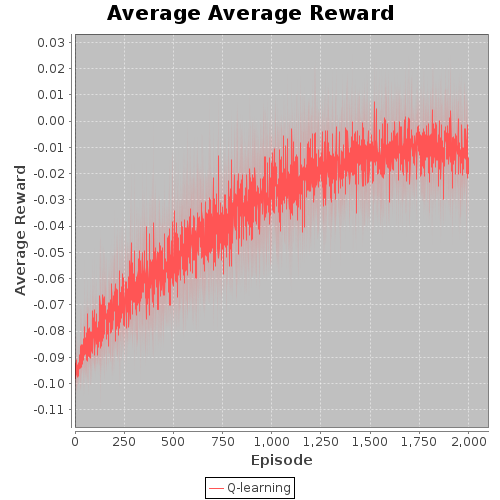
\includegraphics[width=\textwidth]{../graphics/GridWorld_0.3_Q_reward.png}
					\caption{Average reward for GW with initial Q value of 0.3.}
					\label{fig:GW:qinit1}
				\end{subfigure}
				\begin{subfigure}[t]{0.24\textwidth}
					\centering
					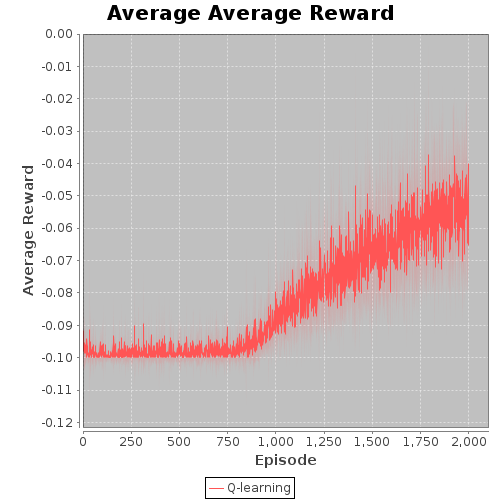
\includegraphics[width=\textwidth]{../graphics/GridWorld_30_Q_rewards.png}
					\caption{Average reward for GW with initial Q value of 30.}
					\label{fig:GW:qintit2}
				\end{subfigure}
				\caption{Average reward for GW with different initial Q values.}
				\label{fig:GW:aqinit}
			\end{figure}

			\begin{figure}[]
				\centering
				\begin{subfigure}[t]{0.24\textwidth}
					\centering
					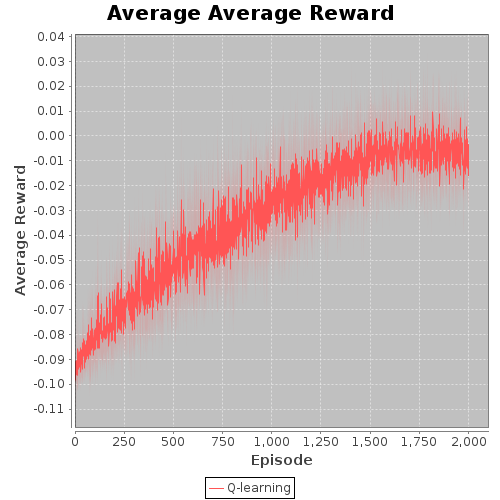
\includegraphics[width=\textwidth]{../graphics/GridWorld_0.05_E_rewards.png}
					\caption{Average reward for GW with epsilon value of 0.05.}
					\label{fig:GW:epsilon1}
				\end{subfigure}
				\begin{subfigure}[t]{0.24\textwidth}
					\centering
					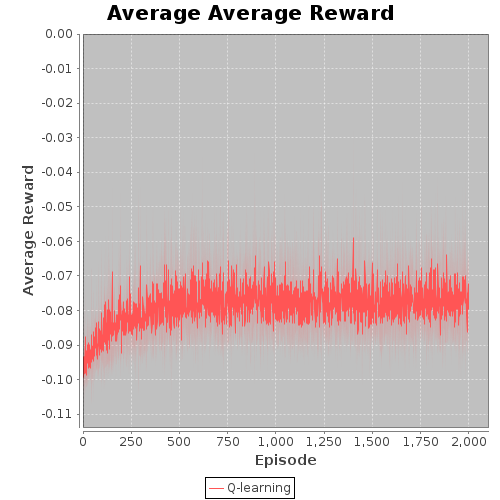
\includegraphics[width=\textwidth]{../graphics/GridWorld_0.8_E_rewards.png}
					\caption{Average reward for GW with epsilon value of 0.8.}
					\label{fig:GW:epsilon2}
				\end{subfigure}
				\caption{Average reward for GW with different epsilon values.}
				\label{fig:GW:aepsilon}
			\end{figure}
		\subsection{Q-Learning - Block Dude}

			\begin{figure}[]
				\centering
				\begin{subfigure}[t]{0.49\textwidth}
					\centering
					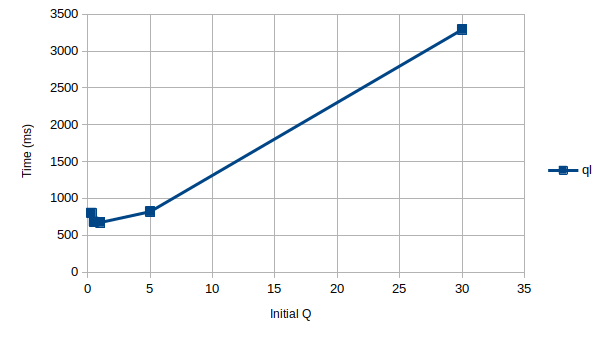
\includegraphics[width=\textwidth]{../graphics/BlockDude_time_q.png}
					\caption{Time according to the initial Q value.}
					\label{fig:BD:qinit}
				\end{subfigure}
				\begin{subfigure}[t]{0.49\textwidth}
					\centering
					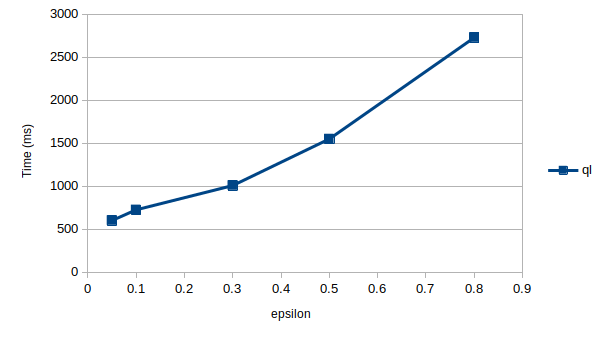
\includegraphics[width=\textwidth]{../graphics/BlockDude_time_epsilon.png}
					\caption{Time according to the epsilon value.}
					\label{fig:BD:epsilon}
				\end{subfigure}
				\begin{subfigure}[t]{0.49\textwidth}
					\centering
					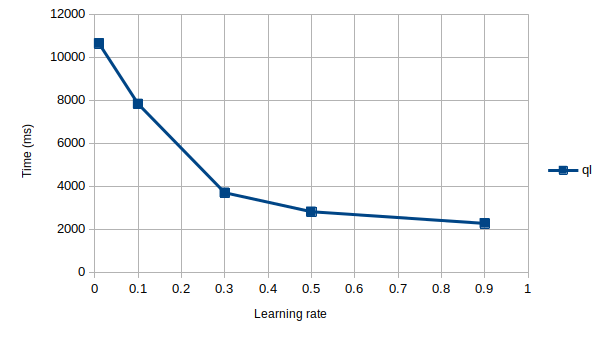
\includegraphics[width=\textwidth]{../graphics/BlockDude_time_rate.png}
					\caption{Time according to the the learning rate.}
					\label{fig:BD:rate}
				\end{subfigure}
				\caption{Number of iterations to converge to an optimal policy according to the parameters of the Grid World problem.}
				\label{fig:BD:QL}
			\end{figure}

			For the BD problem, we also experimented multiple initial Q values and epsilon as shown in figure \ref{fig:BD:QL}. The best performance of initial Q value is 0.3 and worst is 30. The best performance of epsilon value is 0.05 and worst is 0.8. The comparison of these two results are shown in figure \ref{fig:BD:aqinit} and figure \ref{fig:BD:aepsilon}. The best performance appears at the same positions as it does in GW problem. This means that, both problems do no need much exploration. Therefore, we might guess that the result of QL should also be worse than VI and PI. Actually, this depends on the metrics. If we evaluate the performance in terms of reward, then VI and PI for GW is better than QL for GW. As we can see from figure \ref{fig:GW:size:comparison}, most reward values are greater than zero while the result of QL is still smaller than zero. However, if we compare these two methods in terms of run time, then QL is better than PI. Most run time measurements of PI are greater than 10000 ms while QL takes less than 5000 ms. Therefore, I think that, in terms of GW and BD, VI and PI are generally better than QL in terms of reward, while QL is better than PI in terms of run time. Also as we saw, higher initial Q value and higher epsilon value have longer run time. Obviously, this is due to excessive exploration with Q value and high epsilon value.

			For the learning rate parameter, we obtained similar results than in the GW problem, with the exception of that a high learning rate, meaning that the agent considers a lot more the most recent information, does not give bad results.

			\begin{figure}[]
				\centering
				\begin{subfigure}[t]{0.24\textwidth}
					\centering
					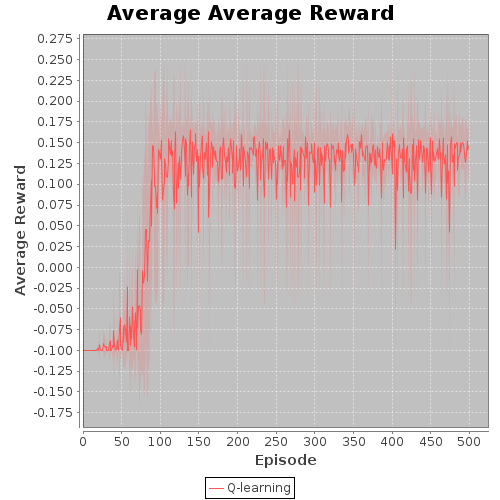
\includegraphics[width=\textwidth]{../graphics/BlockDude_0.3_q.png}
					\caption{Average reward for BD with initial Q value of 0.3.}
					\label{fig:BD:qinit1}
				\end{subfigure}
				\begin{subfigure}[t]{0.24\textwidth}
					\centering
					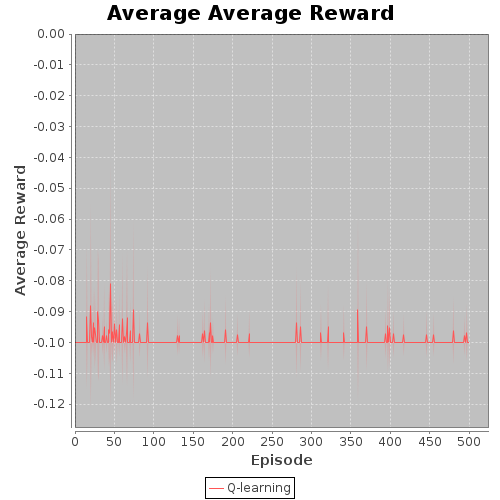
\includegraphics[width=\textwidth]{../graphics/BlockDude_30_q.png}
					\caption{Average reward for BD with initial Q value of 30.}
					\label{fig:BD:qintit2}
				\end{subfigure}
				\caption{Average reward for BD with different initial Q values.}
				\label{fig:BD:aqinit}
			\end{figure}

			\begin{figure}[]
				\centering
				\begin{subfigure}[t]{0.24\textwidth}
					\centering
					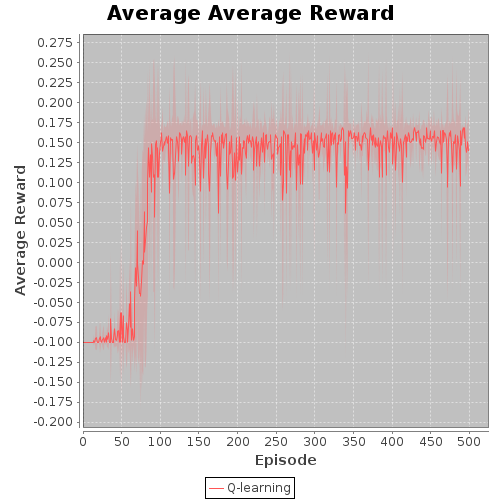
\includegraphics[width=\textwidth]{../graphics/BlockDude_0.05_epsilon.png}
					\caption{Average reward for BD with epsilon value of 0.05.}
					\label{fig:BD:epsilon1}
				\end{subfigure}
				\begin{subfigure}[t]{0.24\textwidth}
					\centering
					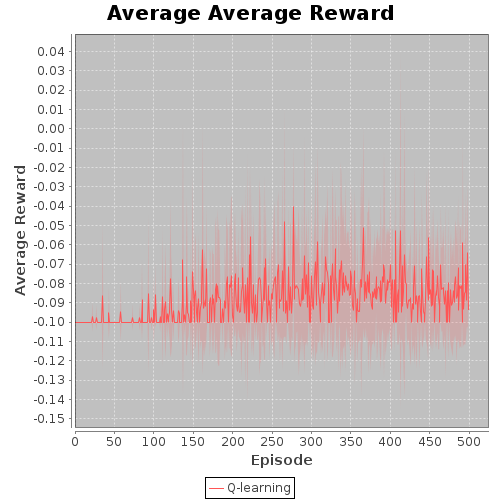
\includegraphics[width=\textwidth]{../graphics/BlockDude_0.8_epsilon.png}
					\caption{Average reward for BD with epsilon value of 0.8.}
					\label{fig:BD:epsilon2}
				\end{subfigure}
				\caption{Average reward for BD with different initial Q values.}
				\label{fig:BD:aepsilon}
			\end{figure}
	\section{Conclusion}
		In conclusion, we saw in that report how worked the different MDP algorithms to solve an MDP and how their parameters can affect the performance of the algorithms. We also saw an reinforcement learning algorithm, Q-Learning and how it can be used to solve an model-free MDP problem.
\end{document}